\subsection{Open short}

\subsubsection{Trader deposit}\label{trader-deposit}
For some number of bonds being shorted, $\Delta y$, the short deposit in shares is made up of several components:

\begin{itemize}
\item The \textbf{total value} that underlies the bonds: $V(\Delta y) = \left( \frac{c_1}{c_0} + \phi_f \right) \cdot \frac{\Delta y}{c}$
\item The \textbf{curve fee}: $\Phi_{\text{c,os}}(\Delta y) = \phi_{c} \cdot (1 - p) \cdot \frac{\Delta y}{c}$
\item The \textbf{short principal}: $L(\Delta y) = z_e - \tfrac{1}{\mu} \cdot (\tfrac{\mu}{c} \cdot (k - (y + \Delta y)^{1 - t_s}))^{\tfrac{1}{1 - t_s}}$
\end{itemize}

where $p$ is the \textbf{spot price}, which defines the relationship between shares and bonds when making an infinitesimally small trade and is given by

\begin{equation}\label{spot-price}
p = \left( \tfrac{\mu \cdot z_e}{y} \right)^{t_s}
\end{equation}

The trader opening a short has to pay a \textbf{deposit}, $D(\Delta y)$, which is their maximum loss when closing the short, or

\begin{equation}\label{short-deposit}
D(\Delta y) =
\begin{cases}
    V(\Delta y) - L(\Delta y) + \Phi_{c,os}(\Delta y),
      & \text{if } V(\Delta y) > L(\Delta y) - \Phi_{c,os}(\Delta y) \\
    0,              & \text{otherwise}
\end{cases}
\end{equation}

The cases avoid situations with negative interest and thus ensure we are trading in a valid regime.
The success case is also defined as the \textbf{short proceeds}, which are the proceeds in shares of closing a short position and are given by

\begin{equation}\label{short-proceeds}
\text{short\_proceeds} = V(\Delta y) - \Delta z = \left( \tfrac{c_1}{c_0} + \phi_f \right) \cdot \tfrac{\Delta y}{c} - \Delta z
\end{equation}

Where $\Delta z = L(\Delta y) - \Phi_{c,os}(\Delta y)$ is the fee-adjusted share delta.
Importantly, this surfaces a constraint that the short principal must be greater than the curve fee for a given $\Delta y$.
Due to the different scaling properties between the non-linear $L(\Delta y)$ and linear $\Phi_{c,os}(\Delta y)$, this constraint is not strictly a function of market parameters, but is also a function of the magnitude of $\Delta y$.

For some deposit, the realized price for the trader is

\begin{equation}\label{realized-price}
p_r = 1 - \frac{D(\Delta y)}{\Delta y}
\end{equation}

LPs take the opposite side of trades, so when a trader opens a short the LP opens a long.
The short principal is the price paid by the LP to buy bonds, which are then set aside as if ``sold'' by the trader when they opened their short.
The price the LP paid is

\begin{equation}\label{lp-price}
p_{l} = \frac{L(\Delta y)}{\Delta y}
\end{equation}

\subsubsection{Open Short Derivatives}

\subsubsubsection{Curve fee}
The curve fee derivative is:

\begin{equation}\label{curve-fee-derivative}
\Phi^{\prime}_{\text{c,os}}(\Delta y) = \tfrac{1}{c} \cdot \phi_{c} \cdot (1 - p)
\end{equation}

\subsubsubsection{Total value}
The total value derivative is also a constant:

\begin{equation}
V^{\prime}(\Delta y) = \tfrac{c_{1}}{c_{0} \cdot c} + \tfrac{\phi_{f}}{c}
\end{equation}

\subsubsubsection{Short principal}\label{short-principal-derivative}
For the short principal derivative, let:

\begin{equation}
u = \frac{\mu}{c} \cdot \left( k - (y + \Delta y)^{1-t_s} \right)
\end{equation}

\begin{equation}
\frac{du}{d \Delta y} = \frac{\mu}{c} \cdot -(1 - t_s) \cdot (y + \Delta y)^{-t_s}
\end{equation}

therefore,

\begin{equation}\label{eq-short-principal-derivative}
\begin{aligned}
L^{\prime}(\Delta y) &= - \frac{1}{\mu} \cdot \frac{1}{1-t_s} \cdot u^{\frac{1}{1-t_s} - 1} \cdot \frac{du}{d \Delta y} \\
&= - \frac{1}{\mu} \cdot \frac{1}{1-t_s} \left( \frac{\mu}{c} \left( k - (y + \Delta y)^{1 - t_s} \right) \right)^{\frac{t_s}{1-t_s}}
\cdot \frac{\mu}{c} \cdot -(1 - t_s) \cdot (y + \Delta y)^{t_s} \\
&= \frac{1}{c} \cdot (y + \Delta y)^{-t_s} \cdot \left( \frac{\mu}{c} \cdot \left( k - (y + \Delta y)^{1 - t_s} \right) \right)^{\frac{t_s}{1 - t_s}}
\end{aligned}
\end{equation}

\subsubsubsection{Short deposit}
Together these give us the short deposit derivative in units of base:

\begin{equation}
D^{\prime}(\Delta y) =
\begin{cases}
    c \cdot \left( V^{\prime}(\Delta y) - L^{\prime}(\Delta y) + \Phi^{\prime}_{\text{c,os}}(\Delta y) \right),
    & \text{if } V(\Delta y) > L(\Delta y) - \Phi_{\text{c,os}}(\Delta y) \\
    0,              & \text{otherwise}
\end{cases}
\end{equation}

Simplifying the condition where the derivative is non-zero, let:

\begin{displaymath}
\begin{aligned}
d &= c \cdot \left( V^{\prime}(\Delta y) - L^{\prime}(\Delta y) + \Phi^{\prime}_{\text{c,os}}(\Delta y) \right) \\
&= c \cdot \left( 
\left( \tfrac{c_{1}}{c_{0} \cdot c} + \tfrac{\phi_{f}}{c} \right)
- \left( \frac{1}{c} \left( \frac{\mu}{c} \cdot \left( k - (y + \Delta y)^{1 - t_s} \right) \right)^{\frac{t_s}{1 - t_s}} \cdot (y + \Delta y)^{-t_s} \right)
+ \left( \phi_{c} \cdot (1 - p) \right) \right) \\
&= 
\tfrac{c_{1}}{c_{0}} + \phi_{f}
- \left( \frac{\mu}{c} \cdot \left( k - (y + \Delta y)^{1 - t_s} \right) \right)^{\frac{t_s}{1 - t_s}} \cdot (y + \Delta y)^{-t_s}
+ c \cdot \phi_{c} \cdot (1 - p) \\
\end{aligned}
\end{displaymath}


\subsubsection{Estimating the maximum possible short}

We must compute the maximum possible short for a given pool in order to provide an upper bound for user trades.

\subsubsubsection{Share reserves after a short}
When a short trade for $\Delta y$ bonds is executed, the Hyperdrive pool's share reserves become:

\begin{equation}\label{reserve-after-max}
    z_1(\Delta y) = \tfrac{1}{\mu}
    \cdot \left( \tfrac{\mu}{c} \cdot \left( k - (y_0 + \Delta y)^{1 - t_s} \right) \right)^{\tfrac{1}{1 - t_s}}
    + \phi_c \cdot (1 - p) \cdot (1 - \phi_g) \cdot \tfrac{\Delta y}{c}
\end{equation}

We will label the left-hand side of the equation as the YieldSpace component and the right-hand side as the fee component.
The final reserve levels for bonds, $y_1 = y_0 + \Delta y$, and shares, $z_1 = z_0 + \Delta z$, result in a net increase in bonds.
The shares typically decrease, but in situations with low spot price and high fees, it is possible that the reduction in shares used to mint bonds is less than the additional shares paid by the trader in the form of fees, resulting in a net increase in pool share reserves.

\subsubsubsection{Minimum share reserves given exposure}

A pool's realized minimum share reserves is a function of the preset minimum constant, $z_{\text{min}}$, the exposure, $e$, and the share adjustment, $\zeta$:

\begin{equation}\label{solvency-constraints}
\begin{aligned}
    z_1 &\ge z_{\text{min}} \\
    z_1 &\ge z_{\text{min}} + \zeta \\
    z_1 &\ge z_{\text{min}} + \tfrac{e}{c}
\end{aligned}
\end{equation}

Exposure is a positive value represented in bonds, which we convert to shares by dividing by the vault share price.
These checks are performed independently, and thus can be combined via max operations: $ z_1 - \text{max}\left( \zeta, \tfrac{e}{c}, 0 \right) \ge z_{\text{min}}$.
When a short is opened, the exposure is reduced by the short bond amount, which impacts the solvency constraint.
To account for this, we can define the exposure after a short, $e_s(\Delta y) = \text{max}(e - \Delta y, 0)$.
With this in mind, our solvency-constrained maximum short is given by:

\begin{equation}\label{pool-min-share-reserves}
\begin{aligned}
    z_{1,\text{min}} = &z_{\text{min}} + \text{max}\left( \zeta, \tfrac{e_s(\Delta y_{\text{max}})}{c}, 0 \right) \\
    = &\tfrac{1}{\mu} \cdot \left(
    \tfrac{\mu}{c} \cdot \left( k - (y_0 + \Delta y_{\text{max}})^{1 - t_s} \right)
    \right)^{\tfrac{1}{1 - t_s}} \\
    &+ \phi_c \cdot (1 - p) \cdot (1 - \phi_g) \cdot \tfrac{\Delta y_{\text{max}}}{c}
\end{aligned}
\end{equation}


From here, we cannot determine a closed-form solution for $\Delta y_{\text{max}}$, but we can approximate it with a linear estimate.

\subsubsubsection{Conservative YieldSpace estimate}

Considering \eqref{pool-min-share-reserves}, we want to compute a linear approximation that underestimates the YieldSpace component, resulting in a smaller estimated $\Delta y$.
This can be achieved via a first-order Taylor Series tangent line approximation, which always lies below the convex YieldSpace curve:

\begin{equation}
\begin{aligned}
    z_{1,ys}(\Delta y) = f(\Delta y) &= \frac{1}{\mu} \left( \frac{\mu}{c} \left( k - \left( y_0 + \Delta y \right)^{1 - t_s} \right)\right)^{\frac{1}{1 - t_s}} \\
    &\ge f(0) + f'(0) \cdot \Delta y
\end{aligned}
\end{equation}

The derivative is computed via the chain rule:

\begin{equation}
\begin{aligned}
    h(\Delta y) &= \frac{\mu}{c} \left( k - \left( y_0 + \Delta y \right)^{1 - t_s} \right) \\
    h'(\Delta y) &= - \frac{\mu}{c} \cdot (1 - t_s) \cdot (y_0 + \Delta y)^{-t_s} \\
    f(\Delta y) &= \frac{1}{\mu} \left( h(\Delta y) \right)^{\frac{1}{1-t_s}} \\
    f'(\Delta y) &= \frac{1}{\mu} \cdot \left( \frac{1}{1 - t_s} \right) \cdot h(\Delta y)^{\frac{t_s}{1 - t_s}} \cdot h'(\Delta y) \\
    &= \frac{1}{\mu} \cdot \left( \frac{1}{1 - t_s} \right) \cdot h(\Delta y)^{\frac{t_s}{1 - t_s}} \cdot \left( - \frac{\mu}{c} \cdot \left( 1 - t_s \right) \cdot \left( y_0 + \Delta y \right)^{-t_s} \right) \\
    &= - \frac{1}{c} \cdot h(\Delta y)^{\frac{t_s}{1 - t_s}} \cdot \left( y_0 + \Delta y \right)^{-t_s} \\
    &= - \frac{1}{c} \cdot \left( \frac{\mu}{c} \left( k - \left( y_0 + \Delta y \right)^{1 - t_s} \right) \right)^{\frac{t_s}{1 - t_s}} \cdot \left( y_0 + \Delta y \right)^{-t_s} \\
    &= -L^{\prime}(\Delta y) \\
    \therefore \\
    f(\Delta y) &\ge \frac{1}{\mu} \left( \frac{\mu}{c} \left( k - (y_0 + 0)^{1-t_s} \right) \right)^{\frac{1}{1 - t_s}} \\
    &- \frac{1}{c} \left( \frac{\mu}{c} \left( k - (y_0 + 0)^{1 - t_s} \right) \right)^{\frac{t_s}{1 - t_s}} \cdot (y_0 + 0)^{-t_s} \cdot \Delta y \\
\end{aligned}
\end{equation}

To simplify the equation, we start from the YieldSpace invariant \eqref{keq}:

\begin{equation}\label{alt-h0}
\begin{aligned}
    k &= \tfrac{c}{\mu} \left( \mu \cdot \left( z_0 - \zeta \right) \right)^{1 - t_{s}} + y_0^{1 - t_{s}} \\
    \therefore \\
    \left( \mu \cdot \left( z_0 - \zeta \right) \right)^{1 - t_s} &= \frac{\mu}{c} \cdot \left( k - y_0^{1-t_s} \right) = h(0)
\end{aligned}
\end{equation}

We can substitute \eqref{alt-h0} into $f(0)$ to get the initial effective share reserves:

\begin{equation}
\begin{aligned}
    f(0) &= \frac{1}{\mu} \left( \frac{\mu}{c} \left( k - y_0^{1-t_s} \right) \right)^{\frac{1}{1 - t_s}} \\
    &= \frac{1}{\mu} h(0)^{\frac{1}{1 - t_s}} \\
    &= \frac{1}{\mu} \left( \left( \mu \cdot \left( z_0 - \zeta \right) \right)^{1 - t_s} \right)^{\frac{1}{1 - t_s}} \\
    &= z_0 - \zeta
\end{aligned}
\end{equation}

We can also substitute \eqref{alt-h0} into $f'(0)$ and write it in terms of the spot price, \eqref{spot-price}:

\begin{equation}
\begin{aligned}
    f'(0) &= - \frac{1}{c} \cdot h(0)^{\frac{t_s}{1 - t_s}} \cdot \ y_0^{-t_s} \\
    &= - \frac{1}{c} \cdot \left( \left( \mu \cdot \left( z_0 - \zeta \right) \right)^{1 - t_s} \right)^{\frac{t_s}{1 - t_s}} \cdot \ y_0^{-t_s} \\
    &= - \frac{1}{c} \left( \frac{\mu \cdot \left( z_0 - \zeta \right)}{y_0} \right)^{t_s} \\
    &= - \frac{p}{c}
\end{aligned}
\end{equation}

This gives us a simplified Taylor approximation to set a bound on the YieldSpace contribution to the maximum short amount:

\begin{equation}\label{approx-f-of-dy}
\begin{aligned}
    z_{1,ys}(\Delta y) &= \frac{1}{\mu} \left( \frac{\mu}{c} \left( k - \left( y_0 + \Delta y \right)^{1 - t_s} \right)\right)^{\frac{1}{1 - t_s}} \\
    &\ge f(0) + f'(0) \Delta y\\
    \therefore\\
    z_{1,ys}(\Delta y) &\ge z_0 - \zeta - \tfrac{p}{c} \cdot \Delta y \\
\end{aligned}
\end{equation}

We can now combine the conservative YieldSpace term with the fee term to get a conservative linear estimate given some short amount, $\Delta y$:

\begin{equation}\label{z1-and-z1est}
\begin{aligned}
    z_1(\Delta y) = &\tfrac{1}{\mu}
    \cdot \left( \tfrac{\mu}{c} \cdot \left( k - (y_0 + \Delta y)^{1 - t_s} \right) \right)^{\tfrac{1}{1 - t_s}} \\
    &+ \phi_c \cdot (1 - p) \cdot (1 - \phi_g) \cdot \tfrac{\Delta y}{c} \\
    \\
    z_{1,\text{est}}(\Delta y) = &z_0 - \zeta - \tfrac{\Delta y}{c} \cdot p + \tfrac{\Delta y}{c} \cdot \phi_c \cdot (1 - p) \cdot (1 - \phi_g) \\
    = &z_0 - \zeta + \tfrac{\Delta y}{c} \cdot \left( \phi_c \cdot (1 - p) \cdot (1 - \phi_g) - p \right)
\end{aligned}
\end{equation}

Together, Equations \eqref{approx-f-of-dy} and \eqref{z1-and-z1est} demonstrate that for some short amount, the actual pool reserve amount is greater than the linear estimate: $z_1(\Delta y) \ge z_{1,\text{est}}(\Delta y)$.
Alternatively, we can find two short amounts that make them equal: $z_{1,\text{min}} = z_1(\Delta y_{\text{max}}) = z_{1,\text{est}}(\Delta y_{\text{est}})$.
The Taylor approximation always lies \emph{below} the YieldSpace curve except at $(z_0, y_0)$, where they are equal.
Therefore, the computed $y_{1,\text{est}}$ for a fixed $z$ must be below the corresponding $y_{1,\text{ys}}$ for the YieldSpace curve.
And thus, $\Delta y_{\text{est}} \le \Delta y_{\text{max}}$.

\newpage

\subsubsubsection{Final linear estimate}\label{conservative-abs-max}

Plugging the minimum share reserves into the approximate equation gives

\begin{equation}
    z_0 - \zeta + \tfrac{\Delta y}{c} \cdot \left( \phi_c \cdot (1 - p) \cdot (1 - \phi_g) - p \right) = z_{\text{min}} + \text{max}\left( \zeta, \tfrac{e_s(\Delta y)}{c}, 0 \right)
\end{equation}

Where again the exposure after a short is $e_s(\Delta y) = \text{max}(e - \Delta y, 0)$.
One solution for handling the non-linearities resulting from the \code{max} functions is to ignore their dependency on $\Delta y$ by assuming an upper-bound on exposure:

\begin{equation}
\begin{split}
    z_0 - \zeta + \tfrac{\Delta y}{c} \cdot \left( \phi_c \cdot (1 - p) \cdot (1 - \phi_g) - p \right) = z_{\text{min}} + \text{max}\left( \zeta, \tfrac{e}{c}, 0 \right)  \\
    \Delta y = \frac{c \cdot \left( z_{\text{min}} + \text{max}\left( \zeta, \tfrac{e}{c}, 0 \right) - \left( z_0 - \zeta \right) \right)}{\phi_c \cdot (1 - p) \cdot (1 - \phi_g) - p}
\end{split}
\end{equation}

However, when exposure is large this overestimate will result in $z_1 > z_0$, which incorrectly implies no short is possible.
Instead, we can break the problem into conditionals.
If $\zeta \ge \tfrac{e}{c}$, then any reduction in exposure due to the short is irrelevant.
The limiting factor is the share adjustment, $\zeta$:

\begin{equation}\label{dy-zeta-limiting}
    \Delta y = \frac{c \cdot \left( z_{\text{min}} + \zeta  - \left( z_0 - \zeta \right) \right)}{\phi_c \cdot (1 - p) \cdot (1 - \phi_g) - p}
\end{equation}

If $\zeta < \tfrac{e}{c}$, then the exposure is the limiting factor, but only while $\tfrac{e - \Delta y}{c} > \zeta$.
If $\Delta y \ge e - c \cdot \zeta$, then Equation \eqref{dy-zeta-limiting} holds.
Otherwise, if $\Delta y < e - c \cdot \zeta$, then we should consider exposure reduction due to the short:

\begin{equation}\label{dy-exposure-limiting}
\begin{aligned}
    z_0 - \zeta + \tfrac{\Delta y}{c} \cdot \left( \phi_c \cdot (1 - p) \cdot (1 - \phi_g) - p \right) &= z_{\text{min}} + \tfrac{e}{c} - \tfrac{\Delta y}{c}  \\
    \tfrac{\Delta y}{c} \cdot \left( \phi_c \cdot (1 - p) \cdot (1 - \phi_g) - p + 1 \right) &= z_{\text{min}} + \tfrac{e}{c} - \left( z_0 - \zeta \right) \\
    \Delta y = \frac{c \cdot \left( z_{\text{min}} + \tfrac{e}{c} - \left( z_0 - \zeta \right) \right)}{\phi_c \cdot (1 - p) \cdot (1 - \phi_g) - p + 1} \\
\end{aligned}
\end{equation}

In practice, we will solve for both of the solutions in Equations \eqref{dy-zeta-limiting} and \eqref{dy-exposure-limiting}, and use the larger of the two that is still solvent.


\subsubsubsection{Estimate visualization}

To understand the impact of the estimate, we can compare against solving the YieldSpace component in isolation, ignoring fees.
To do this, we solve for the bond amount on the curve, $y_{1,ys}$ given the minimum share amount:

\begin{equation}\label{linear-ys-y1}
\begin{aligned}
    k &= \tfrac{c}{\mu} \cdot \left( \mu \cdot \left( z_{1} - \zeta \right) \right)^{1 - t_s} + y_{1,ys}^{1 - t_s} \\
    \therefore \\
    y_{1,ys} &= \left( k - \tfrac{c}{\mu} \cdot \left( \mu \cdot \left( z_{1} - \zeta \right) \right)^{1 - t_s} \right)^{\tfrac{1}{1 - t_s}}
\end{aligned}
\end{equation}

Finally, we can visualize the relationship between these quantities by setting some constants:

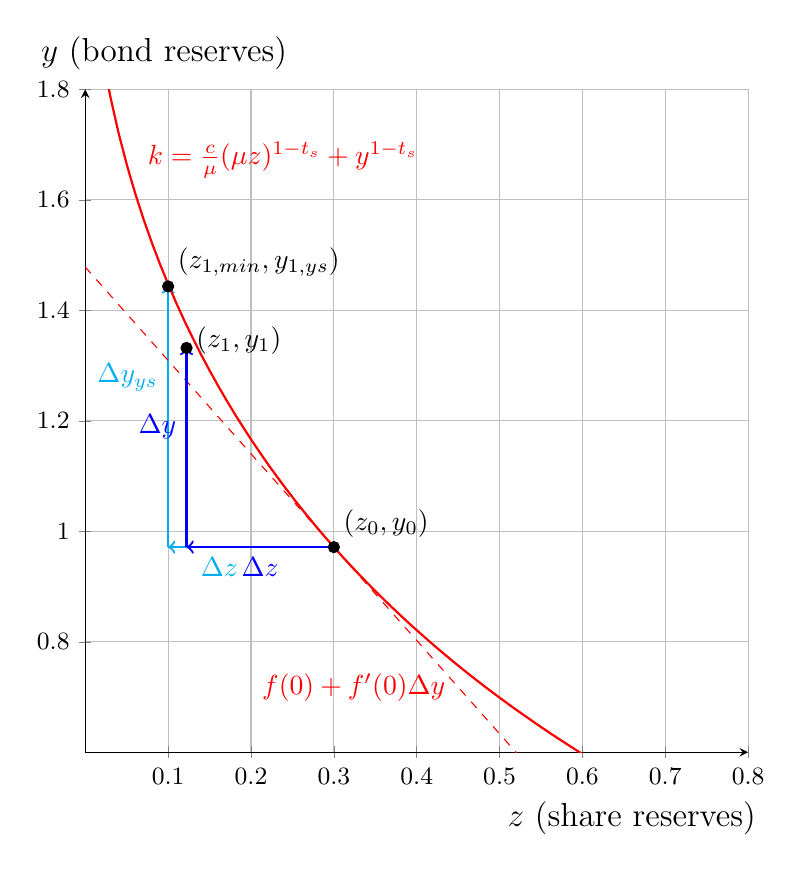
\begin{tikzpicture}
    \begin{axis}[
        xlabel={$z$ (share reserves)},
        ylabel={$y$ (bond reserves)},
        grid=major, % Adds grid lines
        axis lines=middle, % Places the axes in the middle
        width=10cm,
        height=10cm,
        xmin=0, xmax=0.8,
        ymin=0.6, ymax=1.8,
        domain=0:2,
        samples=200, % Number of sample points for smooth curve
        every axis label/.append style={font=\large}, % Makes labels larger
        ticklabel style = {font=\small},
        xlabel style={at={(ticklabel* cs:1.05)}, anchor=north, xshift=-1.9cm, yshift=-0.5cm}, % Moves xlabel outside
        ylabel style={at={(ticklabel* cs:1.05)}, anchor=south, xshift=1.0cm, yshift=-0.3cm}, % Moves ylabel outside
    ]

    % Constants & initial conditions
    \def\k{1.5}
    \def\ts{0.5}
    \def\u{1.5}
    \def\c{1.15}
    \def\phic{0.15}
    \def\phig{0.1}
    \def\zzero{0.3}
    \def\zone{0.1}
    \def\zeta{0.0001}

    % Points y0, y1
    \pgfmathsetmacro{\yzero}{( \k - \c/\u * (\u*\zzero)^(1-\ts) )^(1/(1-\ts))}
    \pgfmathsetmacro{\yone}{( \k - \c/\u * (\u*\zone)^(1-\ts) )^(1/(1-\ts))}
    % Plot points
    \addplot[only marks, mark=*] coordinates {(\zzero,\yzero) (\zone,\yone)};
    % Labels points
    \node[anchor=south west] at (axis cs:\zzero, \yzero) {$(z_0, y_0)$};
    \node[anchor=south west] at (axis cs:\zone, \yone) {$(z_{1,\text{min}}, y_{1,ys})$};
    % Show real ∆y, ∆z
    \draw[cyan, thick, ->] (axis cs:\zzero,\yzero) -- (axis cs:\zone,\yzero) node[midway, below, xshift=-0.4cm] {$\Delta z$};
    \draw[cyan, thick, ->] (axis cs:\zone,\yzero) -- (axis cs:\zone,\yone) node[midway, left, yshift=0.5cm] {$\Delta y_{\text{ys}}$};

    % YieldSpace curve in red
    \addplot[thick, red] 
        { ( \k - \c/\u * (\u * x)^(1-\ts) )^(1/(1-\ts)) };
    % Label for the yieldspace curve
    \def\labelz{0.04}
    \pgfmathsetmacro{\labely}{( \k - \c/\u * (\u*\labelz)^(1-\ts) )^(1/(1-\ts))}
    \node[anchor=north west, red, xshift=0.25cm] at (axis cs:\labelz,\labely) {$k = \frac{c}{\mu}(\mu z)^{1 - t_s} + y^{1 - t_s}$};

    % Compute spot price 'p'
    \pgfmathsetmacro{\p}{ ( (\u * (\zzero - \zeta)) / \yzero )^\ts }

    % Compute slope 'm' of the tangent line at (z0, y0)
    % m = dy/dz = 1 / (dz/dy) = 1 / (-p*/c) = -c/p*
    \pgfmathsetmacro{\m}{ -\c / \p}

    % Plot tangent line at (z0, y0)
    \addplot [dashed, red] { \yzero + \m * (x - \zzero) };
    % Label for the tangent line
    \pgfmathsetmacro{\fprimelabelx}{ 0.4 }
    \pgfmathsetmacro{\fprimelabely}{\yzero + \m * (\fprimelabelx - \zzero)}
    \node[red, xshift=-0.8cm, yshift=-0.6cm] at (axis cs:\fprimelabelx, \fprimelabely) {$f(0) + f'(0) \Delta y$};
    
    % Using the linear approximation to find ~y1
    \pgfmathsetmacro{\tildedeltay}{ (\c * (\zzero - \zeta - \zone)) / (\p - \phic * (1 - \p) * (1 - \phig))}
    \pgfmathsetmacro{\tildeyone}{\yzero + \tildedeltay}
    
    % Define and plot ~z1 for estimated ∆y
    \pgfmathsetmacro{\tildedeltaz}{\zzero - (1 / \u) * ((\u / \c) * (\k - \tildeyone^(1-\ts)))^(1 / (1-\ts)) + \phic * (1 - \p) * (1 - \phig) * (\tildedeltay / \c) }
    \pgfmathsetmacro{\tildezone}{\zzero - \tildedeltaz}
    \addplot[only marks, mark=*] coordinates {(\tildezone, \tildeyone)};
    \node[anchor=south west, yshift=-0.2cm] at (axis cs:\tildezone, \tildeyone) {$(\Tilde{z_1}, \Tilde{y_1})$};
    % Label ~∆z and ~∆y
    \draw[blue, thick, ->] (axis cs:\zzero,\yzero) -- (axis cs:\tildezone,\yzero) node[midway, below] {$\Tilde{\Delta z}$};
    \draw[blue, thick, ->] (axis cs:\tildezone,\yzero) -- (axis cs:\tildezone,\tildeyone) node[left, yshift=-1.00cm] {$\Tilde{\Delta y}$};
    
    \end{axis}
\end{tikzpicture}

\subsubsection{Refining the maximum possible short estimate}\label{newton-refinement}

Starting from the estimate in section \ref{conservative-abs-max}, we will use Newton's Method to refine our guess.
The non-linearity arising from the nested \code{max} functions in equation \eqref{pool-min-share-reserves} creates an additional challenge for refining the estimate using a gradient-base method.
We circumvent this problem by ignoring the exposure in the loss, and checking for it in an early-stopping condition during optimization.
Thus, we define the target share reserves ignoring exposure as $z_t = z_\text{min} + \text{max}(\zeta, 0)$, which is used in our loss function:

\begin{equation}\label{newton-loss}
    l(\Delta y) = z_t - z_1(\Delta y)
\end{equation}

where $z_1(\Delta y)$ is the share reserves after our current max short guess, defined in equation \eqref{reserve-after-max}.
Newton's method also requires the derivative, which we can simplify by writing in terms of the short principal derivative (Equation \eqref{eq-short-principal-derivative}) and curve fee derivative (Equation \eqref{curve-fee-derivative}).

\begin{equation}\label{delta-shares-derivative}
\begin{aligned}
    \frac{d \Delta z}{d \Delta y} &= -L^{\prime}(\Delta y)
        - \Phi^{\prime}_{\text{c,os}}(\Delta y) \cdot (1 - \phi_g) \\
    \therefore \\
    l^{\prime}(\Delta y) &= -\frac{d \Delta z}{d \Delta y} \\
\end{aligned}
\end{equation}

This gives us our Newton update:

\begin{equation}\label{newton-update}
    \Delta y_{n+1} = \Delta y_{n} - \frac{l(\Delta y_{n})}{l^{\prime}(\Delta y_{n})}
\end{equation}

\subsection{Close short}
Closing a short depends on the amount of bonds to be closed, the vault share price when opening the short, the current vault share price, the maturity time of the short, and the current time.
We first compute a normalized time remaining for the bonds:

\begin{equation}\label{normalized-time-remaining}
    \bar{T} = \frac{t_{m} - t_{c}}{d}
\end{equation}

where $t_{m}$ is the maturity time of the short, $t_c$ is the current checkpoint time, and $d$ is the bond position duration.
The pool share delta is made up of a curve component, flat component, and fee component.
The flat component is

\begin{equation}\label{close-short-flat}
    \Delta z_{\text{flat}}(\Delta y) = \frac{\Delta y}{c} \cdot (1 - \bar{T})
\end{equation}

The curve component is

\begin{equation}\label{close-short-curve}
\Delta z_{\text{curve}}(\Delta y) =
\begin{cases}
    \frac{1}{\mu} \cdot \left( \frac{\mu}{c} \cdot k - \left( y_0 - \Delta y \cdot \bar{T}^{-1} \right)^{1-t_s} \right)^{\frac{1}{1 - t_s}} - (z_{0} - \zeta) , & \text{if} \bar{T} > 0 \\
    0, & \text{otherwise}
\end{cases}
\end{equation}

The fee component is

\begin{equation}\label{close-short-fees}
\Delta z_{\text{fees}}(\Delta y) =  \frac{\Delta y}{c} \cdot \left( \phi_c \cdot (1 - p) \cdot \bar{T} + \phi_f \cdot (1 - \bar{T}) \right)
\end{equation}

Together these give the pool share delta:

\begin{equation}\label{close-short-shares-returend}
\Delta z(\Delta y) = \Delta z_{\text{flat}}(\Delta y) + \Delta z_{\text{curve}}(\Delta y) + \Delta z_{\text{fees}}(\Delta y)
\end{equation}

The amount returned to the trader is a function of this pool share delta:

\begin{equation}\label{close-short-trader-return}
    R(\Delta y) =  V(\Delta y) + \phi_f \cdot \frac{\Delta y}{c} - \Delta z(\Delta y)
\end{equation}

where $V(\Delta y)$ is defined in section \ref{trader-deposit} with the ending share price set to the share price at time of closing the short, $c_1 = c$ and $c_0$ is the share price when opening the short.
This return is only valid if the left terms, $V(\Delta y) + \phi_f \cdot \frac{\Delta y}{c}$, are greater than the pool share delta, $\Delta z$.
Otherwise, the user receives zero shares.

\subsubsection{Determining the close short bond amount from a desired return}
It could be the case where a trader wants to determine how many bonds to close to get a certain return back, in shares.
This is an intractable inverse function, much like the max short function.
However, we can follow the same procedure in sections \ref{conservative-abs-max} to produce a linear approximation of the non-linear curve pool share delta term.
Ignoring the condition where the close short returns are zero,

\begin{equation}
\begin{aligned}
    \Delta z_{\text{curve}}(\Delta y) = f(\Delta y) &= 
    \frac{1}{\mu} \cdot \left( \frac{\mu}{c} \cdot k - \left( y_0 - \Delta y \cdot \bar{T}^{-1} \right)^{1-t_s} \right)^{\frac{1}{1 - t_s}} - (z_{0} - \zeta) \\
    &\ge f(0) + f'(0) \cdot \Delta y
\end{aligned} 
\end{equation}

When we evaluate $f(\Delta y)$ at $\Delta y = 0$ we cancel the $\bar{T}$ term.
The additional terms from computing a share delta cancels out the initial effective share reserves, giving us:

\begin{equation}\label{close-short-delta-z-curve-approx}
    \Delta z_{\text{curve}}(\Delta y) \ge \Tilde{\Delta z}_{\text{curve}}(\Delta y) = - \frac{p}{c} \cdot \Delta y
\end{equation}

This was the only non-linear term, so now we can write out our full linear approximation and invert it:

\begin{equation}\label{close-short-delta-z-approx}
\begin{aligned}
    \Tilde{\Delta z}(\Delta y) &= \Delta z_{\text{flat}}(\Delta y) + \Tilde{\Delta z}_{\text{curve}}(\Delta y) + \Delta z_{\text{fees}}(\Delta y) \\
    \therefore \\
    R(\Delta y) &=  V(\Delta y) + \phi_f \cdot \tfrac{\Delta y}{c} - \Delta z(\Delta y) \\
    &\ge \tfrac{\Delta y}{c} \cdot \left( \tfrac{c_1}{c} + 2 \cdot \phi_f - \left(1 - \bar{T} \right) + p - \phi_c \cdot (1 - p) \cdot \bar{T} - \phi_f \cdot \left( 1 - \bar{T} \right) \right) \\
    \therefore \\
    \Delta y \le \Tilde{\Delta y} &= \frac{c \cdot R(\Delta y)}{\tfrac{c_1}{c} + 2 \cdot \phi_f - \left(1 - \bar{T} \right) + p - \phi_c \cdot (1 - p) \cdot \bar{T} - \phi_f \cdot \left( 1 - \bar{T} \right)}
\end{aligned}
\end{equation}

This equation allows us to conservatively approximate the amount of bonds to be shorted, $\Tilde{\Delta y}$, to provide a requested return amount to the trader, $R(\Delta y)$.
As in section \ref{newton-refinement}, we can use Newton's Method to refine the result:

\begin{equation}
\begin{aligned}
    l(\Delta y) &= R_{t}(\Delta y) - R(\Delta y) \\
    l^{\prime}(\Delta y) &= - \frac{d R(\Delta y)}{d \Delta y} \\
    R^{\prime}(\Delta y) &= V^{\prime}(\Delta Y) + \frac{\phi_f}{c} - \Delta z^{\prime}(\Delta y) \\
    \Delta z^{\prime}(\Delta y) &= \Delta z^{\prime}_{\text{curve}}(\Delta y)
    + \frac{1}{c} \cdot
    \left( \bar{T} + \phi_c \cdot (1-p) \cdot \bar{T} + \phi_f \cdot \left(1 - \bar{T}\right) \right)
\end{aligned}
\end{equation}

We will need to follow the procedure in section \ref{short-principal-derivative} to find the derivative $\Delta z^{\prime}_{\text{curve}}(\Delta y)$.
Let,

\begin{equation}
u = \frac{\mu}{c} \cdot \left( k - (y + \Delta y \cdot \bar{T})^{1-t_s} \right)
\end{equation}

\begin{equation}
\frac{du}{d \Delta y} = \frac{\mu}{c} \cdot -(1 - t_s) \cdot \bar{T} \cdot (y + \Delta y \cdot \bar{T})^{-t_s}
\end{equation}

therefore,

\begin{equation}
\begin{aligned}
\Delta z^{\prime}_{\text{curve}}(\Delta y) &= - \tfrac{1}{\mu} \cdot \tfrac{1}{1-t_s} \cdot u^{\tfrac{1}{1-t_s} - 1} \cdot \tfrac{du}{d \Delta y} \\
&= - \tfrac{1}{\mu} \cdot \tfrac{1}{1-t_s} \left( \tfrac{\mu}{c} \left( k - (y + \Delta y \cdot \bar{T})^{1 - t_s} \right) \right)^{\tfrac{t_s}{1-t_s}}
\cdot \tfrac{\mu}{c} \cdot -(1 - t_s) \cdot \bar{T} \cdot (y + \Delta y \cdot \bar{T})^{t_s} \\
&= \tfrac{\bar{T}}{c} \cdot (y + \Delta y \cdot \bar{T})^{-t_s} \cdot \left( \tfrac{\mu}{c} \cdot \left( k - (y + \Delta y \cdot \bar{T})^{1 - t_s} \right) \right)^{\tfrac{t_s}{1 - t_s}}
\end{aligned}
\end{equation}

Given these, the Newton update is the same as Equation \eqref{newton-update}.

\subsection{Targeted short}\label{targeted-short}
TODO